\documentclass[11pt,a4paper]{article}

\usepackage[utf8x]{inputenc}   % omogoča uporabo slovenskih črk kodiranih v formatu UTF-8
\usepackage[slovene]{babel}    % naloži, med drugim, slovenske delilne vzorce

\usepackage[hyphens]{url}
\usepackage{hyperref}

\usepackage{graphicx}


\title{Analiza literature za mojo diplomsko nalogo}
\author{Matic Isovski\\
mi5658@student.uni-lj.si\\
\ \\
predvideni MENTOR: doc. dr. Luka Šajn \\
% za UNI porgram višji predavatelji ne morejo biti mentorji!
Fakulteta za računalništvo in informatiko\\ 
Univerza v Ljubljani
\date{\today}         
}



\begin{document}
\maketitle

\section{Optical music sheet segmentation}

Predstavljen je segmentacijski modul sistema O / sup 3 / MR (objektno orientirano optično prepoznavanje glasbe). Predlagani pristop temelji na sprejetju projekcij za ekstrakcijo osnovnih simbolov, ki predstavljajo grafični element glasbene notacije \cite{omss}.

Najbol citirana publikacija, ki jo obravnavani članek citira je študija o prepoznavi glasbenih znakov \cite{orms}. Najvišji h-index od avtorjev knjige ima A. Rebelo: 47.

V tej študiji pa je najbol citirana knjiga o ujemanju predmetov z uporabo deformabilnih predlog \cite{omudt}. Najvišji h-index od avtorjev knjige ima Anil K. Jain: 188.

Vse članke, knjige, podatke o citiranju ter h-indexu sem pridobival iz strani:
\begin{itemize}
\item
\url{http://eprints.fri.uni-lj.si}
\item
\url{https://scholar.google.com}
\item
\url{https://www.sciencedirect.com}
\item
\url{https://ieeexplore.ieee.org}
\item
\url{https://www.mendeley.com}
\end{itemize}


\section{The Challenge of Optical Music Recognition}

Ta članek \cite{tcomr} opisuje izzive, ki jih predstavlja optično prepoznavanje glasbe. Najprej je opisan problem, nato pa je predstavljen splošen okvir za programsko opremo, ki poudarja ključne točke, ki jih je treba rešiti: identifikacija osebja, prepoznavanje glasbenih predmetov, klasifikacija glasbenih funkcij in glasbena semantika.

Najbol citirana publikacija, ki jo obravnavani članek citira je članek o računalniški grafiki ter pristopih in praksah \cite{cgpp}. Najvišji h-index od avtorjev knjige ima James D. Foley: 41.

V tem članku pa je najbol citiran članek o računalniški grafiki in računalniško generirani vsebini \cite{cgm}. Najvišji h-index od avtorjev knjige ima D.B. Arnold: 20.


\section{Food Object Recognition Using a Mobile Device: State of the Art}

Ta članek \cite{article2} predstavlja devet mobilnih sistemov za prepoznavanja hrane na podlagi njihove sistemske arhitekture in njihovih jedrnih lastnosti.

Najbol citirana publikacija, ki jo obravnavani članek citira je knjiga o izboljševanju Fisher-jevega kernela za klasifikacijo velikih slik \cite{improving}. Najvišji h-index od avtorjev knjige ima Florent Perronnin: 34.

V tem članku pa je najbol citirana knjiga o prepoznavni lastnosti slike \cite{distinctive}. Najvišji h-index od avtorjev knjige ima David Lowe: 51.


\section{Nariši miselni vzorec za svojo diplomsko nalogo}

\begin{figure}[p]
\centerline{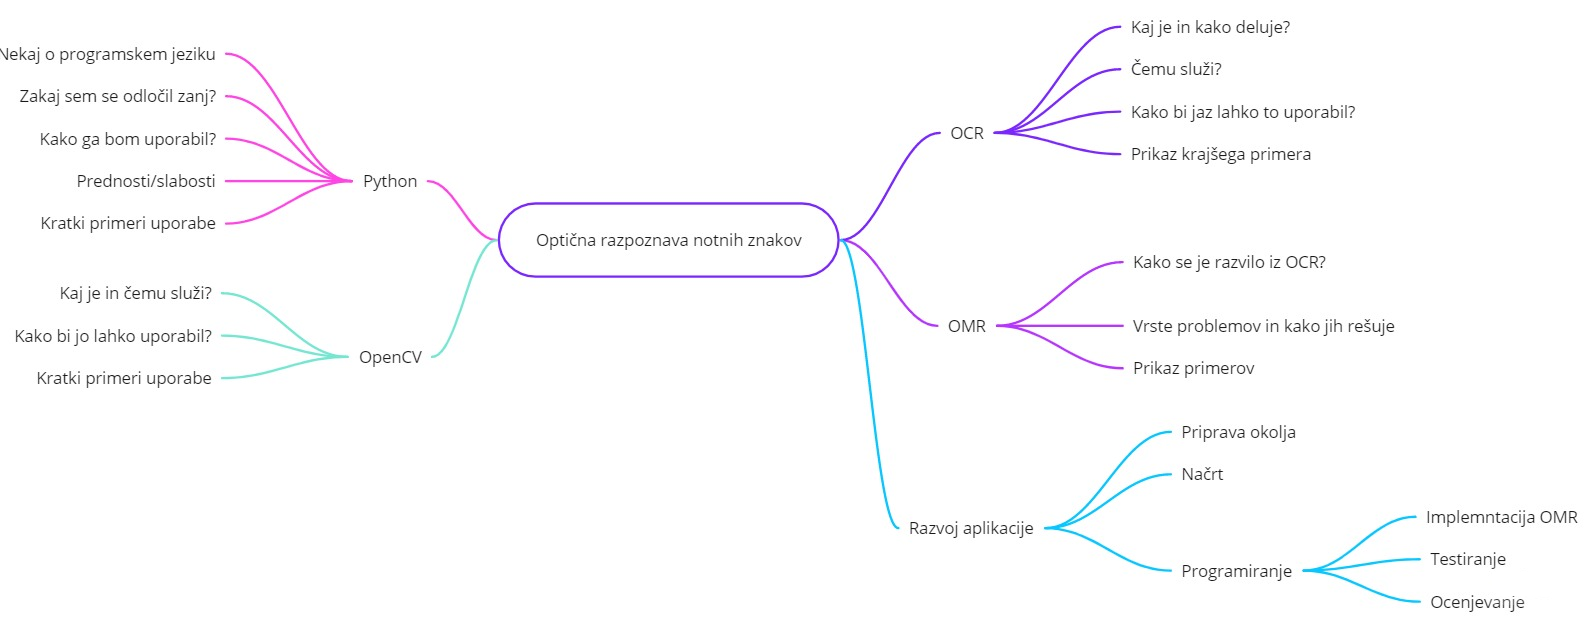
\includegraphics[scale=0.45, angle=90]{mindmap.png}}
\caption{Miselni vzorec za mojo diplomsko nalogo.}
\label{sl:mindmap}
\end{figure}

Na strani 3 lahko vidimo sliko, ki prikazuje miselni vzorec za mojo diplomsko nalogo (Slika \ref{sl:mindmap}). Na hitro lahko vidimo, da je razdeljeno na pet delov: Pytgon (kjer bom pisal o tem programskem jeziku), OpenCV (kjer bom pisal o uporabi te knjižnjice), OMR (kjer bom predstavil tehnologijo optične prepoznave znakov), OCR (kjer bom predstavil podvejo), ter razvoj aplikacije (predstavil bom postopek izdelave aplikacije).



\bibliographystyle{plain}
\bibliography{literatura}

\end{document}  




